\documentclass[../../../main.tex]{subfiles}

\begin{document}
\begin{multicols}{2}[\section{Classical mechanics}]
  \subsection{Motion in one dimension}
  \subsubsection{Integration of Newton's 2nd law}
  \begin{prop}[Newton's 2nd law]
    Consider a particle with constant mass $m$ that moves in one dimension. Then, it satisfies: $$\ddot{x}(t)=\frac{1}{m}F(x(t),\dot{x}(t),t)$$
    where we have supposed the force function $F$ is known and $x(t)$ is the position of the particle as a function of time. We also suppose initial position and velocity, denoted by $x(t_0)=x_0$ and $\dot{x}(t_0)=\dot{x}_0$ respectively, are known.
  \end{prop}
  \begin{prop}[Integration of Newton's 2nd law]
    We consider a force that only depend on time, position and velocity.
    \begin{itemize}
      \item Time dependence:
            \begin{gather*}
              \dot{x}(t)=\dot{x}(t)+\int_{t_0}^t\frac{F(t')}{m}\dd t'\\
              x(t)=x(t_0)+\int_{t_0}^t\dot{x}(t')\dd t'
            \end{gather*}
      \item Position dependence:
            \begin{gather*}
              {\dot{x}(x)}^2={\dot{x}(x_0)}^2+2\int_{x_0}^x\frac{F(x')}{m}\dd x'\\
              x(t)=g^{-1}(t)
            \end{gather*}
            where $\displaystyle g(x)=\int_{x_0}^x\frac{1}{\dot{x}(x')}\dd x'=t$.
      \item Velocity dependence:
            \begin{gather*}
              \dot{x}(t)=h^{-1}(t)\\
              x(t)=x(t_0)+\int_{t_0}^th^{-1}(t')\dd t'
            \end{gather*}
            where $\displaystyle h(\dot{x})=\int_{\dot{x}_0}^{\dot{x}}\frac{m}{F(\dot{x}')}\dd\dot{x}'=t$.
    \end{itemize}
  \end{prop}
  \subsubsection{Variable mass}
  \begin{prop}[Mass accretion formula]
    Consider two objects of masses $m(t)$ and $dm$ and velocities $\vectorfunction{v}(t)$ and $\vectorfunction{u}(t)$ respectively, which in an interval of time $\dd t$ the second one collide with the first one and become a unique object. If $\vectorfunction{F}^\text{ext}$ is the external force acting to the system, we have:
    \begin{equation}
      \vectorfunction{F}^\text{ext}=m\dot{\vectorfunction{v}}+(\vectorfunction{v}-\vectorfunction{u})\dot{m}=\dot{\vectorfunction{p}}-\dot{m}\vectorfunction{u}
      \label{mass}
    \end{equation}
    where $\dot{\vectorfunction{p}}$ is the momentum of the object that gains mass\footnote{The formula is also valid for the case when the object is losing mass, i.e. $\dot{m}<0$.}.
  \end{prop}
  \subsubsection{Rocket motion}
  Consider a rocket moving at a velocity $\vectorfunction{v}$ that expels gas at a velocity $\vectorfunction{c}$ with respect to the rocket to propel itself. Suppose the mass of the rocket is $m(t)$ and $m_0:=m(t_0)$. If $\vectorfunction{u}=\vectorfunction{v}+\vectorfunction{c}$ is the velocity of the gas with respect to an external frame of reference and $\vectorfunction{F}^\text{ext}$ is the net external force acting on the rocket, by equation \eqref{mass} we have:
  $$m\dot{\vectorfunction{v}}=\vectorfunction{F}^\text{ext}+\dot{m}\vectorfunction{c}.$$
  \begin{prop}[Rocket without gravity]
    In this case we have $\vectorfunction{F}^\text{ext}=0$ and if we suppose $\vectorfunction{v}=v\vectorfunction{j}$ and $\vectorfunction{c}=-c\vectorfunction{j}$, we have:
    \begin{equation}
      m\frac{\dd v}{\dd t}=-c\frac{dm}{\dd t}\implies v=c\log\frac{m_0}{m}
      \label{rocket}
    \end{equation}
    Consider now the discrete case, i.e. when the function $\dot{m}$ is not differentiable. For that we can consider instantaneous ejections of $\Delta m=(m_0-m_f)/n$ amount of mass where $m_f$ is the mass of the rocket after $n$ ejections of mass. For this case, we have $$v=c\sum_{k=1}^n\frac{(m_0-m_f)/n}{m_f+k(m_0-m_f)/n}=c\sum_{k=1}^n\frac{\Delta m}{m_f+k\Delta m}\footnote{Obviously if we tend $n$ to infinity we get the equation \eqref{rocket}.}$$
  \end{prop}
  \begin{prop}[Rocket with gravity]
    In this case we have $\vectorfunction{F}^\text{ext}=-mg\vectorfunction{j}$. Suppose $\vectorfunction{v}=v\vectorfunction{j}$, $\vectorfunction{c}=-c\vectorfunction{j}$ and, for simplicity, consider only the case when $\dot{m}=-\beta$, $\beta>0$. Therefore, we obtain:
    \begin{equation}
      m\frac{\dd v}{\dd t}=-mg+c\beta\implies v=c\ln\frac{m_0}{m}-\frac{g}{\beta}(m_0-m)
      \label{rockg1}
    \end{equation}
    Observe that if $m_0g>\beta c$ then $\dd v/\dd t$ will be negative, which is not possible. Therefore in this case the formula is not correct if we are considering the rocket launch. In this case the formula becomes
    \begin{equation}
      v=c\ln\frac{\beta c}{mg}-\frac{g}{\beta}\left(\frac{\beta c}{g}-m\right)
      \label{rockg2}
    \end{equation}
    Because of $\dot{m}=-\beta\implies m(t)=m_0-\beta t$, we can express formulas \eqref{rockg1}, \eqref{rockg2} respectively as:
    \begin{gather*}
      v(t)=c\ln\frac{m_0}{m_0-\beta t}-gt\\
      v(t)=c\ln\frac{\beta c}{m_0g-g\beta t}-gt-\frac{g}{\beta}\left(\frac{\beta c}{g}-m_0\right)
    \end{gather*}
  \end{prop}
  \subsection{Oscillations}
  \subsubsection{Simple harmonic oscillator}
  \begin{prop}
    Consider the differential equation $$\ddot{x}+\omega_0^2 x=0$$ with initial values $x(0)=x_0$ and $\dot{x}(0)=\dot{x}_0$. The general solution is:
    \begin{equation}
      x(t)=x_0\cos\omega_0t+\frac{\dot{x}_0}{\omega_0}\sin\omega_0t=A\cos(\omega_0t+\phi)
      \label{mhs}
    \end{equation} where $\displaystyle A=\sqrt{{x_0}^2+{\left(\frac{\dot{x}_0}{\omega_0}\right)}^2}$ and $\displaystyle \phi=-\arctan\frac{\dot{x}_0}{\omega_0x_0}$. Such constants $\omega_0$ ($[\omega_0]=\text{rad}\cdot \text{s}^{-1}$), $A$ ($[A]=\text{m}$) and $\phi$ ($[\phi]=\text{rad}$) are called \textit{angular frequency}, \textit{amplitude} and \textit{initial phase}, respectively. Observe that the function in equation \eqref{mhs} is periodic with period $T=\frac{2\pi}{\omega_0}$ and frequency $\nu=T^{-1}=\frac{\omega_0}{2\pi}$\footnote{Note that $[T]=\text{s}$ and $[\nu]=\text{s}^{-1}=\text{Hz}$.}.
  \end{prop}
  \begin{definition}
    Let $U(x)$ be a potential function of class $\mathcal{C}^2(\mathbb{R})$. We say $x_0$ is a \textit{point of stable equilibrium} if $U$ attains a minimum in $x_0$. Analogously, we say $x_0$ is a \textit{point of unstable equilibrium} if $U$ attains a maximum in $x_0$.
  \end{definition}
  \begin{prop}[Behaviour near a minimum]
    Suppose $x_0$ is a point of stable equilibrium an let $U(x)$ be the potential function associated with a particle of mass $m$. Then if we disturb slightly the particle, it will start to oscillate at a frequency $$\omega_0=\sqrt{\frac{U''(x_0)}{m}}.$$
  \end{prop}
  \begin{prop}[Examples]
    \hfill
    \begin{itemize}
      \item Mass hanging from a spring: Let $y(t)$ be the position of the mass measured from initial string's length (without the mass) to the position of the mass at time $t$. If we disturb the system with an external force so that the mass starts to oscillate, we have $$y(t)=\frac{mg}{k}+A\cos(\omega_0t+\phi),\quad\omega_0=\sqrt{\frac{k}{m}}.$$
            \begin{minipage}{\linewidth}
              \centering
              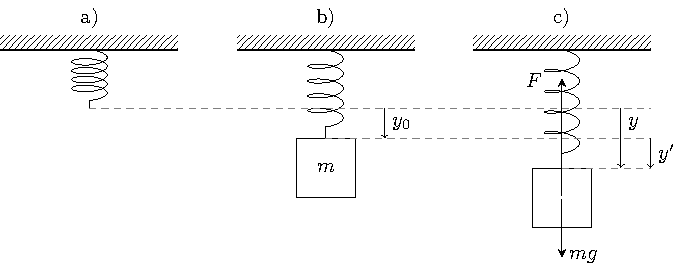
\includegraphics[width=\linewidth]{Physics/2nd/Classical_mechanics/Images/springs.tex}
              \captionof{figure}{Mass hanging from a spring.}
            \end{minipage}
      \item Simple pendulum: $$\theta(t)=A\cos(\omega_0t+\phi),\quad\omega_0=\sqrt{\frac{g}{l}}.$$
            \begin{minipage}{\linewidth}
              \centering
              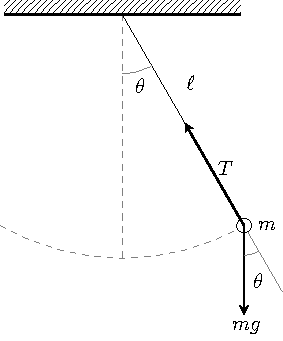
\includegraphics[width=0.5\linewidth]{Physics/2nd/Classical_mechanics/Images/simple_pendulum.tex}
              \captionof{figure}{Simple pendulum.}
            \end{minipage}
      \item Physical pendulum:
            $$\theta(t)=A\cos(\omega_0t+\phi),\quad\omega_0=\sqrt{\frac{mgD}{I_e}}.$$
            \begin{minipage}{\linewidth}
              \centering
              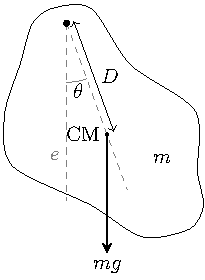
\includegraphics[width=0.5\linewidth]{Physics/2nd/Classical_mechanics/Images/physical_pendulum.tex}
              \captionof{figure}{Physical pendulum.}
            \end{minipage}
      \item LC circuit: $$q(t)=A\cos(\omega_0t+\phi),\quad\omega_0=\frac{1}{\sqrt{LC}}.$$
    \end{itemize}
  \end{prop}
  \subsubsection{Damped harmonic oscillator}
  \begin{prop}[Movement equation]
    Consider the following differential equation: $$\ddot{x}+2\beta\dot{x}+\omega_0^2 x=0,$$ with initials values of $x(0)=x_0$ and $\dot{x}(0)=\dot{x}_0$. Then we have three cases for the general solution:
    \begin{itemize}
      \item If $\beta<\omega_0$,
            \begin{equation}
              x(t)=e^{-\beta t}\left(c_1\cos\Tilde{\omega}t+c_2\sin\Tilde{\omega}t\right).
              \label{b<w}
            \end{equation}
      \item If $\beta=\omega_0$,
            \begin{equation}
              x(t)=e^{-\beta t}\left(c_1+c_2t\right).
              \label{b=w}
            \end{equation}
      \item If $\beta>\omega_0$,
            \begin{equation}
              x(t)=c_1e^{-(\beta+\Tilde{\omega})t}+c_2e^{-(\beta-\Tilde{\omega})t}.
              \label{b>w}
            \end{equation}
    \end{itemize}
    Here $c_1,c_2$ are constants depending on the initial values and we have defined $\displaystyle \Tilde{\omega}=\sqrt{\left|\omega_0^2-\beta^2\right|}$.
  \end{prop}
  \begin{prop}[Energy of damped harmonic oscillator]
    $$E=\frac{\mu}{2}\left(\dot{x}^2+\omega_0^2x^2\right),$$ where $\mu$ is a constant.
  \end{prop}
  \begin{prop}[Underdamped harmonic oscillator: $\beta<\omega_0$]
    Coefficients $c_1,c_2$ of the general solution \eqref{b<w} are: $$c_1=x_0,\quad c_2=\frac{\dot{x}_0+\beta x_0}{\Tilde{\omega}}.$$ The equation, can be simplified to $$x(t)=Ae^{-\beta t}\cos(\Tilde{\omega}t+\phi),$$ where $\displaystyle A=\sqrt{x_0^2+\left(\frac{\dot{x}_0+\beta x_0}{\Tilde{\omega}}\right)^2}$ and\\ $\displaystyle\phi=-\arctan\frac{\dot{x}_0+\beta x_0}{\Tilde{\omega}x_0}$.
  \end{prop}
  \begin{definition}[Quality factor]
    The \textit{quality factor} is defined as follows: $$Q:=\frac{\omega_0}{2\beta}.$$
  \end{definition}
  \noindent From that, we can rewrite the expression of $\Tilde{\omega}$ to get: $$\Tilde{\omega}=\omega_0\sqrt{1-\frac{1}{4Q^2}}.$$
  \begin{prop}[Energy of underdamped harmonic oscillator]
    For
    $$E(t)=\frac{\mu\omega_0^2A^2}{2}e^{-2\beta t}=E_0e^{-2\beta t}.$$ The rate at which the energy is dissipated is $$\left|\frac{dE}{\dd t}(t)\right|=2\beta E(t)\implies\frac{E}{\left|dE/\dd t\right|}=\frac{1}{2\beta}.$$
    If $\beta\ll\omega_0$, then $$Q=2\pi\frac{E}{\Delta E},$$ where $\Delta E$ is the energy dissipated in a pseudo-period $\Tilde{T}=2\pi/\Tilde{\omega}\approx2\pi/\omega_0$.
  \end{prop}
  \begin{prop}[Critically damped harmonic oscillator: $\beta=\omega_0$]
    Coefficients $c_1,c_2$ of the general solution \eqref{b=w} are: $$c_1=x_0,\quad c_2=x_0\omega_0+\dot{x}_0.$$ This harmonic oscillator is the one that returns to balance more quickly.
  \end{prop}
  \begin{prop}[Overdamped harmonic oscillator: $\beta<\omega_0$]
    Coefficients $c_1,c_2$ of the general solution \eqref{b>w} are: $$c_1=\frac{x_0(\Tilde{\omega}-\beta)-\dot{x}_0}{2\Tilde{\omega}},\quad c_2=\frac{x_0(\Tilde{\omega}+\beta)+\dot{x}_0}{2\Tilde{\omega}}.$$
  \end{prop}
  \subsubsection{Driven harmonic oscillators}
  \begin{prop}[Movement equation]
    Consider the following differential equation: $$\ddot{x}+2\beta\dot{x}+\omega_0^2 x=f(t)=f_0\cos(\omega t+\psi),$$ with initials values of $x(0)=x_0$ and $\dot{x}(0)=\dot{x}_0$. Then the particular solution is:
    $$x_p(t)=A\cos(\omega t+\psi-\phi),$$
    where $\displaystyle A=\frac{f_0}{\sqrt{{(\omega_0^2-\omega^2)}^2+4\beta^2\omega^2}}$ and\\ $\displaystyle\phi=\arctan{\frac{2\beta\omega}{\omega_0^2-\omega^2}}$. Therefore for the general solution we have three cases to consider:
    \begin{itemize}
      \item If $\beta<\omega_0$,
            \begin{equation}
              x(t)=e^{-\beta t}(c_1\cos\Tilde{\omega}t+c_2\sin\Tilde{\omega}t)+A\cos(\omega t+\psi-\phi).
              \label{d-b<w}
            \end{equation}
      \item If $\beta=\omega_0$,
            \begin{equation}
              x(t)=e^{-\beta t}\left(c_1+c_2t\right)+A\cos(\omega t+\psi-\phi).
              \label{d-b=w}
            \end{equation}
      \item If $\beta>\omega_0$,
            \begin{equation}
              x(t)=c_1e^{-(\beta+\Tilde{\omega})t}+c_2e^{-(\beta-\Tilde{\omega})t}+A\cos(\omega t+\psi-\phi).
              \label{d-b>w}
            \end{equation}
    \end{itemize}
    Here $c_1,c_2$ are constants depending on the initial values.
  \end{prop}
  \begin{prop}[Underdamped driven oscillator]
    Coefficients $c_1,c_2$ of the general solution \eqref{d-b<w} are:
    \begin{gather*}
      c_1=x_0-A\cos\left(\psi-\phi\right),\\
      c_2=\frac{\dot{x}_0-\omega A\sin\left(\psi-\phi\right)+\beta\left[x_0-A\cos\left(\psi-\phi\right)\right]}{\tilde{\omega}}.
    \end{gather*}
  \end{prop}
  \begin{prop}[Critically damped driven oscillator]
    Coefficients $c_1,c_2$ of the general solution \eqref{d-b=w} are:
    \begin{gather*}
      c_1=x_0-A\cos\left(\psi-\phi\right),\\
      c_2=\dot{x}_0A+\omega_0x_0+A\left(\omega\sin\left(\phi-\psi\right)-\omega_0\cos\left(\psi-\phi\right)\right).
    \end{gather*}
  \end{prop}
  \begin{prop}[Overdamped driven oscillator]
    Coefficients $c_1,c_2$ of the general solution \eqref{d-b>w} are:
    \begin{equation*}
      \begin{split}
        \begin{multlined}[t]
          c_1=A\frac{(\beta-\Tilde{\omega})\cos\left(\psi-\phi\right)-\omega\sin\left(\psi-\phi\right)}{2\Tilde{\omega}}+\\+\frac{-(\beta-\Tilde{\omega})x_0-\dot{x}_0}{2\Tilde{\omega}},
        \end{multlined}\\
        \begin{multlined}[t]
          c_2=A\frac{-(\beta+\Tilde{\omega})\cos\left(\psi-\phi\right)+\omega\sin\left(\psi-\phi\right)}{2\Tilde{\omega}}+\\+\frac{(\beta+\Tilde{\omega})x_0+\dot{x}_0}{2\Tilde{\omega}}.
        \end{multlined}
      \end{split}
    \end{equation*}
  \end{prop}
  \begin{definition}
    Given a driven oscillator, we say it is in the \textit{steady-state part} if $t\gg 1/\beta$. In that case $x(t)$ become: $$x(t)=A\cos(\omega t+\psi-\phi).$$ While the dependency on $c_1,c_2$ is non-negligible, we say the driven oscillator is in the \textit{transient part}.
  \end{definition}
  \begin{prop}[Resonance in amplitude]
    If $\omega=\omega_r:=\sqrt{\omega_0^2-2\beta^2}$ we say the oscillator is in \textit{resonance in amplitude}. For $\omega=\omega_r$ we have $$A_r=\frac{f_0}{2\beta\sqrt{\omega_0^2-\beta^2}}.$$
  \end{prop}
  \begin{prop}[Energy in steady-state part]
    $$E=\frac{\mu A^2}{2}\left[\omega^2\sin^2(\omega t+\psi-\phi)+\omega_0^2\cos^2(\omega t+\psi-\phi)\right].$$ If $\omega\approx\omega_0$ and $\beta\ll\omega_0$ then $$E=\frac{\mu f_0^2}{8}\frac{1}{(\omega-\omega_0)^2+\beta^2}.$$ Observe $E$ has a maximum at $\omega=\omega_0$ with the value of $E^\text{max}=\frac{\mu f_0^2}{8\beta^2}$.
  \end{prop}
  \begin{definition}
    We define the \textit{cutoff frequencies} as this two frequencies: $$\omega_1=\omega_0-\beta,\quad\omega_2=\omega_0+\beta.$$ The value  $\Delta\omega=\omega_2-\omega_1=2\beta$ is called the \textit{bandwidth}. Therefore, we can redefined the quality factor as: $$Q=\frac{\omega_0}{2\beta}=\frac{\omega_0}{\Delta\omega}=\frac{\nu_0}{\Delta\nu}$$
  \end{definition}
  \textcolor{green}{FALTA COSA.}
  \begin{prop}[Impulsive forces]
    Consider a driven oscillator of equation $\ddot{x}+2\beta\dot{x}+\omega_0^2x=f$, where $$f(t)=\left\{
      \begin{array}{cc}
        0   & \text{if } t<t'                    \\
        f_0 & \text{if }t'\leq t\leq t'+\Delta t \\
        0   & \text{if } t>t'+\Delta t
      \end{array}\right.$$
  \end{prop}
  \textcolor{green}{FALTA COSA.}
  \subsection{Central forces}
  \subsubsection{Definition and properties}
  \begin{definition}[Central force]
    A \textit{central force} is a force of the form $$\vectorfunction{F}(\boldsymbol{r})=f(r)\boldsymbol{e}_r,$$ where $r=\|\boldsymbol{r}\|$ and $\boldsymbol{e}_r=\boldsymbol{r}/r$ is the unit radial vector.
  \end{definition}
  \begin{definition}
    The origin $\boldsymbol{r}=0$ is called \textit{center of forces}.
  \end{definition}
  \begin{prop}
    All central forces are conservative and $$f(r)=-U'(r),$$ where $U(r)$ is the potential energy of the central force.
  \end{prop}
  \subsubsection{Conservation of angular momentum and areal velocity}
  \begin{prop}
    The angular momentum with respect to the center of forces is conserved, that is, $\dot{\boldsymbol{L}}=0$.
  \end{prop}
  \begin{prop}[Kepler's 2nd law]
    The areal velocity $dA/\dd t$ is constant. In fact, $$\frac{dA}{\dd t}=\frac{L}{2m}.$$
  \end{prop}
  \begin{prop}[Unit vectors]
    Remember we have $$\boldsymbol{e}_r=\boldsymbol{i}\cos\theta+\vectorfunction{j}\sin\theta,\quad\boldsymbol{e}_\theta=-\boldsymbol{i}\sin\theta+\vectorfunction{j}\cos\theta.$$ Therefore we obtain,
    \begin{equation}
      \boldsymbol{r}=r\boldsymbol{e}_r,\quad\boldsymbol{\dot{r}}=\dot{r}\boldsymbol{e}_r+r\dot{\theta}\boldsymbol{e}_\theta,\quad\boldsymbol{\ddot{r}}=(\ddot{r}-r\dot{\theta}^2)\boldsymbol{e}_r+(2\dot{r}\dot{\theta}+r\ddot{\theta})\boldsymbol{e}_\theta.
      \label{unit}
    \end{equation}
  \end{prop}
  \begin{prop}[Trajectory equation]
    From \eqref{unit}, Newton's second law can be written as: $$\ddot{r}-r\dot{\theta}^2=\frac{f(r)}{m},\quad 2\dot{r}\dot{\theta}+r\ddot{\theta}=0.$$ And we can obtain the following differential equations: $$\dot{\theta}=\frac{L}{m r^2}:=\frac{l}{r^2},\quad\ddot{r}-\frac{l^2}{r^3}=\frac{f(r)}{m},$$ where we have defined the magnitude $l:=L/m$. Finally, we get the \textit{trajectory equation}: $$\frac{d^2}{d\theta^2}\left(\frac{1}{r}\right)+\frac{1}{r}=-\frac{1}{ml^2}r^2f(r).$$
  \end{prop}
  \subsubsection{Conservation of energy and orbits}
  \begin{prop}[Kinetic energy]
    $$K=\frac{1}{2}m|\boldsymbol{\dot{r}}^2=\frac{1}{2}m\dot{r}^2+\frac{ml^2}{2r^2}.$$
  \end{prop}
  \begin{definition}
    We define the effective potential as $$U_\text{eff}=U(r)+\frac{ml^2}{2r^2}.$$ The term $ml^2/(2r^2)$ gives the centripetal force: $$f_\text{centr}=-\frac{d}{dr}\left(\frac{ml^2}{2r^2}\right)\implies\boldsymbol{f}_\text{centr}=mr\dot{\theta}^2\boldsymbol{e}_r$$
  \end{definition}
  \begin{prop}[Energy]
    \begin{equation}
      E=\frac{1}{2}m\dot{r}^2+U_\text{eff}=\frac{1}{2}m\dot{r}^2+\frac{ml^2}{2r^2}+U(r).
      \label{energy}
    \end{equation}
  \end{prop}
  \begin{prop}[Orbits]
    The minimum of $U_\text{eff}(r)$ determines the radius of the \textit{stable circular orbits}. If $E<0$, the orbits are in a range of radius $r_\text{min}$ and $r_\text{max}$, and so are \textit{bounded orbits}. If $E>0$, the orbits are called \textit{unbounded orbits}. Equating equation \eqref{energy} to, we can obtain the angle $\Delta\theta$ in a \textit{radial oscillation}:\footnote{A radial oscillation is the trajectory when $r$ moves from $r_\text{min}$ to $r_\text{max}$ and the comes back to $r_\text{min}$.} $$\Delta\theta=2\int_{r_\text{min}}^{r_\text{max}}\frac{l/r^2}{\sqrt{(2/m)(E-U_\text{eff}}}dr.\footnote{Here we have taken the positive orientation, that is, $\boldsymbol{L}$ pointing to the positive $z$-axis.}$$ Note, that the orbits are \textit{closed orbits} if $$\Delta\theta=2\pi\frac{p}{q},\quad p,q\in\mathbb{N}.$$
  \end{prop}
  \begin{theorem}[Bertrand's theorem]
    The two unique potentials for which every bounded orbit is closed are: $$U(r)=-\frac{k}{r},\quad U(r)=\frac{k}{2}r^2,\quad k>0.$$
  \end{theorem}
  \subsubsection{Potential $-k/r$}
  \begin{prop}[Movement equation]
    $$r(\theta)=\frac{\alpha}{\varepsilon\cos\theta+\text{sgn}\,k},$$where $\displaystyle\alpha=\frac{L^2}{m|k|}$ and $\displaystyle\varepsilon=\sqrt{1+\frac{2EL^2}{mk^2}}$. This is the equation of a conic.
  \end{prop}
  \begin{definition}
    We define the \textit{pericenter of an orbit} as the minimum value of $r(\theta)$, that is, $r=r_\text{min}$. Analogously, we define the \textit{apocenter of an orbit} as the maximum value of $r(\theta)$, that is, $r=r_\text{max}$.
  \end{definition}
  \subsubsection{Conics}
\end{multicols}
\end{document}